\documentclass[11pt]{article}

\usepackage{amsfonts}
\usepackage{graphicx}
\usepackage{listings}

\usepackage{algorithm}
\usepackage{algorithmic}

\begin{document}
\title{DeepDCF: The best feature for the DCF based tracker \\
DCFNet: Discriminant Correlation Filter Network on Visual Tracking\\
Best Convolutional Features for Correlation Filter based Visual Tracking}
\author{QiangWang}
\date{\today}
\maketitle

\section{Abstract}

Discriminative Correlation Filters(DCF) have been widely used recent years in visual tracking due to the high precision and fast training and detection.

Convolutional Networks can enjoy millions labeled images for the offline representation learning.Classification even loss the spatial information.

Tracking is differenet with detection and classification. Classification and DET both eliminate the differences in the same class. 

To put the tracking problem simple to the similarity metrics for total offline learning is a unreasonable hypothesis. The surrounding and the target motion fusing in temporal jointly determine the trajectory of the target.

\section{Introduction}


\subsection{related work}

\subsection{CNN}
	CNN can be  treated as a encode function $ \Phi (x)$ of receptive field.
	
\textit{	\begin{center}
\includegraphics[width=3in]{./img/depthcol.jpg}
\end{center}}
	
$$ \Phi(x)=f^{l} $$
$x \in \mathbb{R}^{m \times n} \longrightarrow f \in \mathbb{R}^{d}$

It is sparse (only a few input units contribute to a given output unit) and reuses parameters (the same weights are applied to multiple locations in the input)

\subsection{contributions}

\section{Discriminative Correlation Filters}
	\subsection{DSST Derivation}
	\textbf{(PCA-HOG+Gray)+DCF+Scale Esimation}\\
	key word: circular correlation,Parserval's identity, dense feature
		\subsubsection{Single Feature(gray)}
		patch: $x_1,...,x_t$	\\
		label: $y_1,...,y_t$	\\
		filter: $w_t$	\\
		test patch: $z$	\\

$$
\epsilon =  \sum_{j=1}^{t}\left \| w_{t}\star x_{j}-y_{j} \right \|^{2} = \sum_{j=1}^{t}\left \| \overline{W}_{t} \odot X_{j}-Y_{j} \right \|^{2}
$$


$$
W_{t}=\frac{\sum_{j=1}^{t}\overline{Y}_{j} \odot X_{j}}{\sum_{j=1}^{t}X_{j} \odot\overline{ X_{j}}} 
$$

$$
y=\mathfrak{F}^{-1} \left( {\overline{W}_{t} \odot Z}\right)
 = \mathfrak{F}^{-1} \left(\frac{\sum_{j=1}^{t}\overline{X}_{j} \odot Y_{j} \odot Z}{\sum_{j=1}^{t}\overline{X_{j}} \odot X_{j}} \right)
$$

This is a little different between MOSSE\cite{MOSSE} and this Derivation. No regularization term.

\subsubsection{Multidimensional Features}

patch: 
$  f^{l} ,l\in \{ 1,...,d \} $
label: 
$ g $
filter: 
$ h^{l} $
test patch: 
$ z^{l} $

$$
\epsilon =  \sum_{l=1}^{d}\left \| h^{l}\star f^{l}-g \right \|^{2} +\lambda \sum_{l=1}^{d}\left\|h^{l} \right\|^{2}
$$

$$
H^{l}=\frac{\overline{G}F^{l}}{\sum_{k=1}^{d}\overline{F^{k}}F^{k}+\lambda}
$$


To obtain a robust approximation, here we update the numerator $A_ {t}^{l} $ and denominator $ B_{t} $

$$
A_{t}^{l} = (1-\eta )A_{t-1}^{l}+\eta \overline{G}_{t}F_{t}^{l}
$$

$$
B_{t}^{l} = (1-\eta )B_{t-1}^{l}+\eta \sum_{k=1}^{d}\overline{F}_{t}F_{t}^{l}
$$

$$
y=\mathfrak{F}^{-1}\left\{ \frac{\sum_{l=1}^{d}\overline{A^{l}}Z^{l}}{B+\lambda}\right\}
$$


	\subsection{CN}


	\subsection{SRDCF}
	\subsection{CF2}

	
	\section{DeepDCF}
	
 The network in this filed utilize pooling to reduce the computation complexity and eliminate the spatial information.
 So we rebuild the network with zero stride and total small size kernel convnet. We think the resolution in the spatial must be reserved. For the shortcomings of no stride and pooling, we have a small receptive field. So we anlynsis use the DilatedNet.
	
	
target patch: $ x^{l} ,l\in \{ 1,...,d \} $
idea label: $ y $
filter: $ w^{l} $
test patch: $ z^{l} $
test output: $ g $

For the learing part.
$$
\epsilon =  \sum_{l=1}^{d}\left \| w^{l}\star x^{l}-y \right \|^{2} +\lambda \sum_{l=1}^{d}\left\|w^{l} \right\|^{2}
$$

$$
W^{l}=\frac{\overline{Y} \odot X^{l}}{\sum_{k=1}^{d}\overline{X^{k}} \odot X^{k}+\lambda}
$$


$$
g=\mathfrak{F}^{-1}\left\{ \frac{\sum_{l=1}^{d}\overline{A^{l}} \odot Z^{l}}{B+\lambda}\right\}
$$

$$
g=\mathfrak{F}^{-1}\left\{ \frac{\sum_{l=1}^{d}\overline{A^{l}} \odot Z^{l}}{B+\lambda}\right\} 
=\mathfrak{F}^{-1}\left\{\frac{ \sum_{l=1}^{d}\overline{\overline{Y} \odot X^{l}} \odot Z^{l}}{\sum_{k=1}^{d}\overline{X^{k}} \odot X^{k}+\lambda}\right\} 
=\mathfrak{F}^{-1}\left\{\frac{ \sum_{l=1}^{d}(Z^{l} \odot \overline{X^{l}}) \odot Y}{\sum_{k=1}^{d}\overline{X^{k}} \odot X^{k}+\lambda}\right\}
$$


\begin{lstlisting}[language=Octave]

g=ifft2((sum(fft2(z).*conj(fft2(x)), 3).*fft2(y))./...
	(sum(fft2(x).*conj(fft2(x)), 3)+lambda)));

\end{lstlisting}

The forward pass derivation should be familiar to us by now. There need some 
patience for the backward pass.

First, let's begining with  some fundamental theorems of DFT and Complex-Valued Derivatives.

Because the DFT is a linear opreator, it's gradient is simply the transformation matrix it self. During the back-progation, then, the gradient is conjugated.\cite{SpectralPool}

$$
Y=\mathfrak{F}\left\{y\right\},\frac{\partial l}{\partial Y} = \mathfrak{F}\left\{\frac{\partial l}{\partial y}\right\}
$$


The second theorem we will use is Complex-Valued Derivatives\cite{Complexderivatives}. Because we need pass $\delta$ throught the frequency domain. We will be more familar with the derivatives operator about complex . Two base formula we should revisited.

Let$ z = x + yi \in \mathbb {C} $represent a complex scalar variable, where $ Re(z) = x $and $ Im(z) = y $ . The following four relations hold between the real and imaginary parts of z and its complex conjugate $ z^{*}$ :

\begin{eqnarray*}
z = x + iy\\
z^{*} = x - iy\\
x = \frac{x+x^{*}}{2}\\
y = \frac{x-x^{*}}{2i}
\end{eqnarray*}

For complex differentials, these four relations can be formulated as follows:

\begin{eqnarray*}
dz = dx + idy\\
dz^{*} = dx - idy\\
dx = \frac{dx+dx^{*}}{2}\\
dy = \frac{dx-dx^{*}}{2i}
\end{eqnarray*}

$$
\frac{\partial f(x)}{\partial x}
$$

$$
\frac{\partial f(x,x^{*})}{\partial x}=\overline{\frac{\partial f(x,x^{*})}{\partial x^{*}}}
$$
 
Now, Let's derive the formulas about the backward. For simplify, We start with 
 $ \frac{\partial l}{\partial g} $ and what we need is to results of  $ \frac{\partial l}{\partial x} $ and $ \frac{\partial l}{\partial z} $.

$$
G_{uv}=\frac{\sum_{l=1}^{d}(Z_{uv}^{l}\overline{X_{uv}^{l}})Y_{uv}}{\sum_{k=1}^{d}X_{uv}^{k}\overline{X_{uv}^{k}}+\lambda}
$$

$$
\frac{\partial l}{\partial Z_{uv}^{l}}=\frac{\partial l}{\partial G_{u,v}}\frac{\partial G_{u,v}}{\partial Z_{uv}}=\mathfrak{F}\left\{\frac{\partial l}{\partial g}\right\}_{uv}  \frac{\overline{X_{uv}^{l}}Y_{uv}}{\sum_{k=1}^{d}X_{uv}^{k}\overline{X_{uv}^{k}}+\lambda}
$$

$$
\frac{\partial l}{\partial X_{uv}^{l}}
=\frac{\partial l}{\partial G_{u,v}}\frac{\partial G_{u,v}}{\partial X_{uv}}
=\mathfrak{F}\left\{\frac{\partial l}{\partial g}\right\}_{uv}
\frac{
\overline{Z_{uv}^{l}Y_{uv}}(\sum_{k=1}^{d}\overline{X_{uv}^{k}}X_{uv}^{k}+\lambda)-\overline{X_{uv}^{k}}(\sum_{l=1}^{d}(Z_{uv}^{l}\overline{X_{uv}^{l}})Y_{uv})}
{(\sum_{k=1}^{d}\overline{X_{uv}^{k}}X_{uv}^{k}+\lambda)^{2}}
$$
	
$$
\frac{\partial l}{\partial x_{uv}^{l}}
=\mathfrak{F}^{-1} \left\{ \frac{\partial l}{\partial X}\right\}_{uv}^l
$$


\begin{algorithm}
\caption{Forward pass: Calculate $y$}
\begin{algorithmic} 
\REQUIRE target $x$, search $z$,initlize position $p$,ConvNet $\Phi(\cdot)$
\RETURN $y$

 \FOR{$i:=1$ \TO $n$}
 \STATE {crop and feature} 
  \STATE {detection and update} 
 \ENDFOR
\end{algorithmic}
\end{algorithm}



\begin{algorithm}
\caption{Backward propagation: Calculate $\Phi(\cdot)$}
\begin{algorithmic} 
\REQUIRE Gradient output$\frac{\partial l}{\partial y}$
\RETURN Gradient input$\frac{\partial l}{\partial x}$,$\frac{\partial l}{\partial z}$

\end{algorithmic}
\end{algorithm}




\section{Experiments}

I think that is a very perfect visualization of the training process.

%\begin{center}
%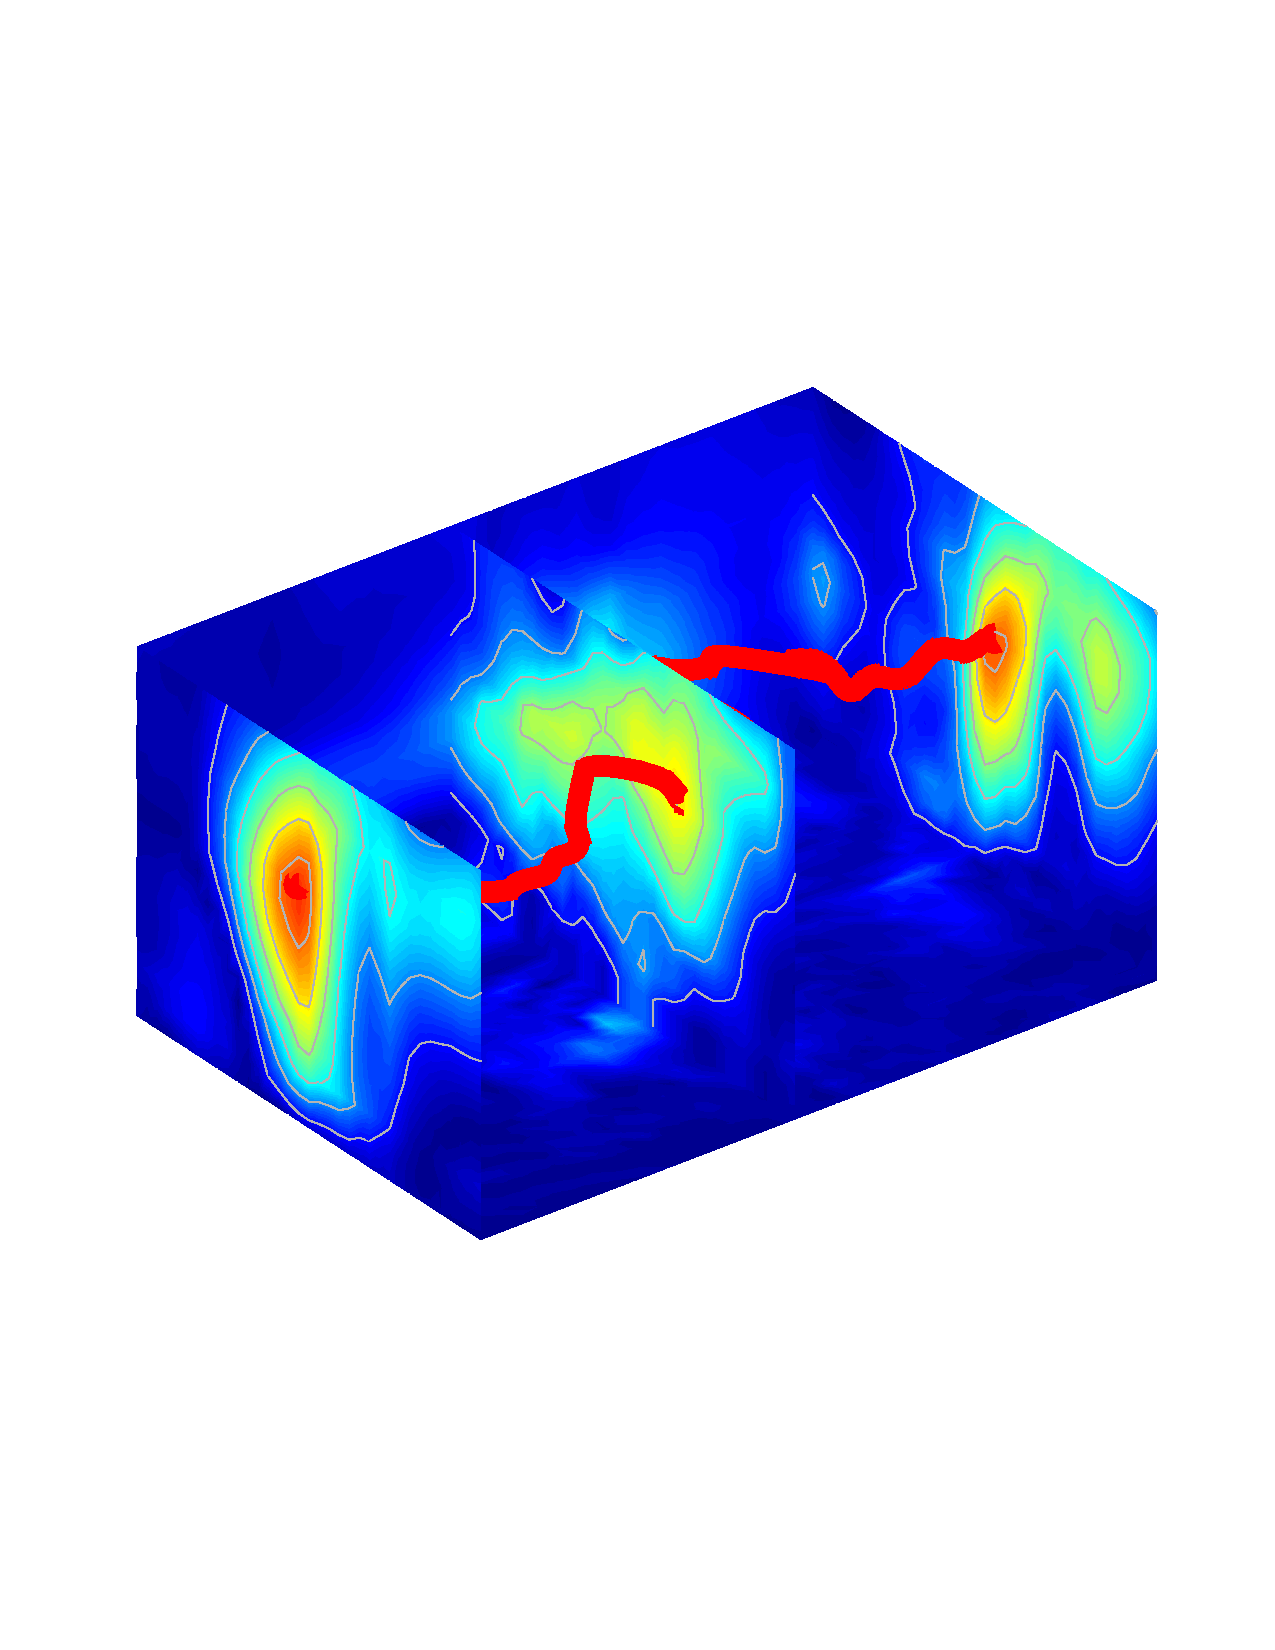
\includegraphics[width=4in,trim = 0mm 65mm 0mm 65mm, clip]{./img/visual_training.pdf}
%\end{center}

\subsection{Details and Paramemters}


\subsection{Baseline Comparison}
Compare with handcraft feature.
Compare different vgg(from shallow to deep)
Compare different receptive field.
Compare different Network(Alex,VGG,ResNet,tingNet)
Compare different memory cost for the net struct.


\subsection{OTB}
In this benchmark,we should pay attention to raw results. Even We can training a very deep network like ResNet.

\subsection{VOT}
In this part, we should pay more attention in speed. 

AR rank 
(EAO  vs speed)  should be presented.


\section{Conclusions}
We are the first to achieve end-to-end learning in DCF.

\pagebreak		
\bibliographystyle{plain}
\bibliography{bibfile}

\end{document}



